% cls && pdflatex cmp.tex && cls && pdflatex cmp.tex && start cmp.pdf
\documentclass[a5paper, 10pt]{article}
\usepackage[T2A,T1]{fontenc}
\usepackage[utf8]{inputenc}
\usepackage[english, ukrainian]{babel}
\usepackage{amsmath, amssymb}
\usepackage[top = 2 cm, left = 1 cm, right = 1 cm, bottom = 2 cm]{geometry} 

\usepackage{fancyhdr}
\pagestyle{fancy}
\lhead{Основи методів обчислень}
\cfoot{\thepage}

\allowdisplaybreaks
\setlength\parindent{0pt}
\numberwithin{equation}{subsection}

\title{{\Huge ОСНОВИ МЕТОДІВ ОБЧИСЛЕНЬ}}
\date{}

\usepackage{xcolor}
\usepackage{hyperref}
\hypersetup{unicode=true,colorlinks=true,linktoc=all,linkcolor=violet}

\usepackage{float, graphicx}
\usepackage{amsthm}
\newtheorem{lemma}{Лема}
\newtheorem*{lemma*}{Лема}
\newtheorem{theorem}{Теорема}
\newtheorem*{theorem*}{Теорема}
\newtheorem{definition}{Визначення}
\newtheorem*{definition*}{Визначення}
\theoremstyle{definition}
\newtheorem{remark}{Зауваження}
\newtheorem*{remark*}{Зауваження}
\newtheorem{example}{Приклад}
\newtheorem*{example*}{Приклад}
\newtheorem{problem}{Задача}
\newtheorem*{problem*}{Задача}
\newtheorem{solution}{Розв'язок}
\newtheorem*{solution*}{Розв'язок}
\newtheorem{corollary}{Наслідок}
\newtheorem*{corollary*}{Наслідок}

\newcommand{\RR}{\mathbb{R}}
\newcommand{\CC}{\mathbb{C}}
\newcommand{\Min}{\displaystyle\min\limits}
\newcommand{\Max}{\displaystyle\max\limits}
\newcommand{\Sup}{\displaystyle\sup\limits}
\newcommand{\Sum}{\displaystyle\sum\limits}
\newcommand{\Prod}{\displaystyle\prod\limits}
\newcommand{\Int}{\displaystyle\int\limits}
\newcommand{\Iint}{\displaystyle\iint\limits}
\newcommand{\Lim}{\displaystyle\lim\limits}

\newcommand*\diff{\mathop{}\!\mathrm{d}}

\renewcommand{\bf}[1]{\textbf{#1}}
\renewcommand{\epsilon}{\varepsilon}
\renewcommand{\phi}{\varphi}

\DeclareMathOperator{\diam}{diam}
\DeclareMathOperator{\rang}{rang}
\DeclareMathOperator{\const}{const}
\DeclareMathOperator{\cond}{cond}

\newenvironment{system}{\begin{equation} \left\{\begin{aligned}}{\end{aligned} \right. \end{equation}}
\newenvironment{system*}{\begin{equation*} \left\{\begin{aligned}}{\end{aligned} \right. \end{equation*}}

\makeatletter
\newcommand*{\relrelbarsep}{.386ex}
\newcommand*{\relrelbar}{%
  \mathrel{%
    \mathpalette\@relrelbar\relrelbarsep
  }%
}
\newcommand*{\@relrelbar}[2]{%
  \raise#2\hbox to 0pt{$\m@th#1\relbar$\hss}%
  \lower#2\hbox{$\m@th#1\relbar$}%
}
\providecommand*{\rightrightarrowsfill@}{%
  \arrowfill@\relrelbar\relrelbar\rightrightarrows
}
\providecommand*{\leftleftarrowsfill@}{%
  \arrowfill@\leftleftarrows\relrelbar\relrelbar
}
\providecommand*{\xrightrightarrows}[2][]{%
  \ext@arrow 0359\rightrightarrowsfill@{#1}{#2}%
}
\providecommand*{\xleftleftarrows}[2][]{%
  \ext@arrow 3095\leftleftarrowsfill@{#1}{#2}%
}
\makeatother

\begin{document}

\maketitle \thispagestyle{empty} \newpage 

У ваших руках конспект лекцій з нормативного курсу ``Основи методів обчислень'', прочитаного доц., к.ф.-м.н. Риженком Андрієм Івановичем на третьому курсі спеціальності прикладна математика факультету комп'ютерних наук та кібернетики Київського національного університету імені Тараса Шевченка восени 2018-го року. \\

Конспект у компактній формі відображає матеріал курсу, допомагає сформувати загальне уявлення про предмет вивчення, правильно зорієнтуватися в даній галузі знань. Конспект лекцій з названої дисципліни сприятиме більш успішному вивченню дисципліни, причому більшою мірою для студентів заочної форми, екстернату, дистанційного та індивідуального навчання. \\

Комп'ютерний набір та верстка -- Скибицький Нікіта Максимович. \newpage

\tableofcontents \newpage

\section{Аналіз похибок заокруглення}

\subsection{Види похибок}

Нехай необхідно розв’язати рівняння
\begin{equation}
	\label{eq:1.1}
	Au = f.
\end{equation}
За рахунок неточно заданих вхідних даних насправді ми маємо рівняння
\begin{equation}
	\label{eq:1.2}
	\tilde A \tilde u = \tilde f.
\end{equation}
Назвемо $\delta_1 = u - \tilde u$ -- \textit{неусувною похибкою}. \\

Застосування методу розв‘язання \eqref{eq:1.2} приводить до рівняння
\begin{equation}
	\label{eq:1.3}
	\tilde A_h \tilde u_h = \tilde f_h,
\end{equation}
де $h > 0$ -- малий параметр. Назвемо $\delta_2 \tilde u - \tilde u_h$ -- \textit{похибкою методу}. \\

Реалізація методу на ЕОМ приводить до рівняння
\begin{equation}
	\label{eq:1.4}
	\tilde A_h^* \tilde u_h^* = \tilde f_h^*.
\end{equation}
Назвемо $\delta_3 = \tilde u_h^* - \tilde u_h$ -- \textit{похибкою заокруглення}. \\

Тоді \textit{повна похибка} $\delta = u - \tilde u_h^* = \delta_1 + \delta_2 + \delta_3$. \\

\begin{definition}
	Кажуть, що задача \eqref{eq:1.1} \textit{коректна}, якщо
	\begin{enumerate}
		\item $\forall f \in F$ $\exists! u \in U$;
		\item задача \eqref{eq:1.1} \textit{стійка}, тобто
		\begin{equation}
			\label{eq:1.5}
			\forall \epsilon > 0 \quad \exists \delta > 0: \|A-\tilde A\| < \delta, \|f-\tilde f\| < \delta \Rightarrow \|u - \tilde u\| < \epsilon.
		\end{equation}
	\end{enumerate}
\end{definition}

Якщо задача \eqref{eq:1.1} \textit{некоректна}, то або розв‘язок її не існує, або він неєдиний, або він нестійкий, тобто 
\begin{equation}
	\label{eq:1.6}
	\exists \epsilon > 0: \forall \delta > 0: \exists A, f: \| A - \tilde A\|<\delta, \|f-\tilde f\| < \delta, \|u-\tilde u\| > \epsilon.
\end{equation}

\textit{Абсолютна похибка} $\Delta (x^*) \ge \max_x |x - x^*|$. \\

\textit{Відносна похибка} $\delta (x^*) \ge \max_x \Delta (x^*) / |x^*|$. \\

\textit{Значущими цифрами} називаються всі цифри, починаючи з першої ненульової зліва. \\

\textit{Вірна цифра} -- це значуща, якщо абсолютна похибка за рахунок відкидання всіх молодших розрядів не перевищує одиниці розряду цієї цифри. Тобто, якщо 
\begin{equation}
	\label{eq:1.7}
	x^* = \overline{\alpha_n \ldots \alpha_0.\alpha_{-1}\ldots\alpha_{-p}\ldots},
\end{equation}
то $\alpha_{-p}$ -- вірна, якщо $\Delta (x^*) \le 10^{-p}$. \\

Інколи $\Delta (x^*) \le w \cdot 10^{-p}$, $1/2 \le w < 1$, наприклад, $w = 0.55$.

\subsection{Підрахунок похибок в ЕОМ}

Підрахуємо відносну похибку заокруглення числа $x$ на ЕОМ з плаваючою комою. В $\beta$-ічній системі числення число представляється у вигляді
\begin{equation}
	\label{eq:1.8}
	x = \pm (\alpha_1 \beta^{-1} + \alpha_2 \beta^{-2} + \ldots + \alpha_t \beta^{-t} + \ldots) \beta^p,
\end{equation}
де $0 \le \alpha_k < \beta$, $\alpha_1 \ne 0$, $k = 1,2,\ldots$ \\

Якщо в ЕОМ $t$ розрядів, то при відкиданні молодших розрядів ми оперуємо з наближеним значенням 
\begin{equation}
	\label{eq:1.9}
	x^* = \pm (\alpha_1 \beta^{-1} + \alpha_2 \beta^{-2} + \ldots + \alpha_t \beta^{-t}) \beta^p,
\end{equation}
і відповідно похибка заокруглення 
\begin{equation}
	\label{eq:1.9_1}
	x - x^* = \pm \beta^p (\alpha_{t+1} \beta^{-t-1} + \ldots)
\end{equation}
Тоді її можна оцінити так
\begin{multline}
	\label{eq:1.10}
	|x - x^*| \le \beta^{p-t-1} \cdot (\beta-1) \cdot (1 + \beta^{-1}+\ldots)\le\\
	\le \beta^{p-t-1} \cdot (\beta-1) \cdot \dfrac{1}{1-\beta^{-1}}=\beta^{p-t}.
\end{multline}

Якщо в представлені \eqref{eq:1.8} взяти $\alpha_1 = 1$, то $|x| \ge \beta^p \cdot \beta^{-1}$. Звідси остаточно 
\begin{equation}
	\label{eq:1.11}
	\delta (x^*) \le \dfrac{\beta^{p-t}}{\beta^{p-1}}=\beta^{1-t}.
\end{equation}

При більш точних способах заокруглення можна отримати оцінку $\delta (x^*) \le \beta^{1-t} / 2 = \epsilon$. Число $\epsilon$ називається ``машинним іпсилон''. Наприклад, для $\beta = 2$, $t = 24$, $\epsilon = 2^{-24} \approx 10^{-7}$.

\subsection{Підрахунок похибок обчислення значення функції}

Нехай задана функція 
\begin{equation}
	\label{eq:1.11_1}
	y = f(x_1, \ldots, x_n) \in C^1(\Omega)
\end{equation}
Необхідно обчислити її значення при наближеному значенні аргументів 
\begin{equation}
	\label{eq:1.11_2}
	\vec x^* = (x_1^*, \ldots, x_n^*),
\end{equation}
де $|x_i - x_i^*| \le \Delta (x_i^*)$ та оцінити похибку обчислення значення функції
\begin{equation}
	\label{eq:1.11_3}
	y^* = f(x_1^*, \ldots, x_n^*).
\end{equation}

Маємо 
\begin{equation}
	\label{eq:1.12}
	|y-y^*| = |f\left(\vec x\right) - f\left(\vec x^*\right)| = \left| \Sum_{i=1}^n \dfrac{\partial f}{\partial x_i} \left(\vec \xi\right) (x_i - x_i^*) \right| \le \Sum_{i=1}^n B_i \cdot \Delta (x_i^*), 
\end{equation}
де 
\begin{equation}
	\label{eq:1.13}
	B_i = \Max_{\vec x \in U} \left| \dfrac{\partial f}{\partial x_i}\left(\vec x\right) \right|.
\end{equation}

Тут 
\begin{equation}
	\label{eq:1.14}
	U = \left\{ \vec x = (x_1, \ldots, x_n): |x_i - x_i^*| \le \Delta (x_i^*)\right\} \in \Omega, \quad i=\overline{1,n}.
\end{equation}
Отже
\begin{equation}
	\label{eq:1.15}
	\Delta (y^*) = |y - y^*| \prec \Sum_{i=1}^n n_i \cdot \Delta (x_i^*),
\end{equation}
з точністю до величин першого порядку малості по
\begin{equation}
	\label{eq:1.15_1}
	\Delta (x^*) = \Max_{i=\overline{1,n}} \Delta (x_i^*),
\end{equation}
де
\begin{equation}
	\label{eq:1.16}
	b_i = \left| \dfrac{\partial f}{\partial x_i}\left(\vec x^*\right) \right|
\end{equation}
та ``$\prec$'' означає приблизно менше. \\

\subsubsection{Похибки арифметичних операцій}

\begin{enumerate}
	\item Сума: $y = x_1 + x_2$, $x_1, x_2 > 0$, 
	\begin{equation}
		\label{eq:1.17}
		\begin{aligned}
		\Delta (y^*) &\le \Delta (x_1^*) + \Delta (x_2^*), \\ 
		\delta (y^*) &\le \dfrac{\Delta (x_1^*) + \Delta (x_2^*)}{x_1^* + x_2^*} \le \max\{\delta (x_1^*), \delta (x_2^*)\}.
		\end{aligned}
	\end{equation}
	
	\item Різниця: $y = x_1 - x_2$, $x_1 > x_2 > 0$,
	\begin{equation}
		\label{eq:1.18}
		\begin{aligned}
		\Delta (y^*) &\le \Delta (x_1^*) + \Delta (x_2^*), \\
		\delta (y^*) &\le \dfrac{x_2^* \delta (x_1^*) + (x_1^*) \delta (x_2^*)}{x_1^* - x_2^*}.
		\end{aligned}
	\end{equation}
	
	При близьких $x_1^*$, $x_2^*$ зростає відносна похибка (за рахунок втрати вірних цифр).

	\item Добуток: $y = x_1 \cdot x_2$, $x_1, x_2 > 0$,
	\begin{equation}
		\label{eq:1.19}
		\begin{aligned}
		\Delta (y^*) &\prec x_2^* \Delta (x_1^*) + x_1^* \Delta (x_2^*), \\
		\delta (y^*) &\le \delta (x_1^*) + \delta (x_2^*).
		\end{aligned}
	\end{equation}

	\item Частка: $y = \dfrac{x_1}{x_2}$, $x_1, x_2 > 0$,
	\begin{equation}
		\label{eq:1.20}
		\begin{aligned}
		\Delta (y^*) &\prec \dfrac{x_2^* \Delta (x_1^*) + x_1^* \Delta (x_2^*)}{(x_2^*)^2}, \\
		\delta (y^*) &\le \delta (x_1^*) + \delta (x_2^*).
		\end{aligned}
	\end{equation}

	При малих $x_2^*$ зростає абсолютна похибка (за рахунок зростання результату ділення). 
\end{enumerate}

\subsection{Обернена задача аналізу позибок}

Нагадаємо, що \textit{пряма задача} аналізу похибок полягає у обчисленні $\Delta (y^*), \delta (y^*)$ по заданих $\Delta (x_i^*)$, $i = \overline{1, n}$. \\

\textit{Обернена задача} полягає у знаходженні $\Delta (x_i^*)$, $i = \overline{1, n}$ по заданих $\Delta (y^*)$, $\delta (y^*)$. Якщо $n > 1$, маємо одну умову 
\begin{equation}
	\label{eq:1.21}
	\Sum_{i=1}^n b_i \Delta (x_i^*) < \epsilon
\end{equation}
для багатьох невідомих $\Delta (x_i^*)$. Вибирають їх із однієї з умов 
\begin{equation}
	\label{eq:1.22}
	b_i \Delta (x_i^*) < \dfrac{\epsilon}{n},
\end{equation}
або
\begin{equation}
	\label{eq:1.23}
	\Delta (x_i^*) < \dfrac{\epsilon}{\Sum_{i=1}^n b_i}.
\end{equation}

\section{Нелінійні рівняння}

\textit{Постановка задачі}. Нехай маємо рівняння $f(x) = 0$, $\overline{x}$ -- його розв’язок, тобто $f (\overline{x}) \equiv 0$. \\

Задача розв‘язання цього рівняння розпадається на етапи:
\begin{enumerate}
	\item Існування та кількість коренів.
	\item Відділення коренів, тобто розбиття числової вісі на інтервали, де знаходиться один корінь.
	\item Обчислення кореня із заданою точністю $\epsilon$.
\end{enumerate}

Для розв'язання перших двох задач використовуються методи математичного аналізу та алгебри, а також графічний метод. Далі розглядаються методи розв'язання третього етапу.

\subsection{Метод ділення навпіл}

Припустимо на $[a, b]$ знаходиться лише один корінь рівняння 
\begin{equation}
	\label{eq:2.1}
	f(x) = 0,
\end{equation}
для $f(x) \in C([a,b])$, який необхідно визначити. Нехай $f(a) \cdot f (b) < 0$. \\

Припустимо, що $f(a) > 0$, $f(b) < 0$. Покладемо $x_1 = \frac{a + b}{2}$ і підрахуємо
$f(x_1)$. Якщо $f_1(x) < 0$, тоді шуканий корінь $x$ знаходиться на інтервалі $(a, x_1)$. Якщо ж $f_1(x) > 0$, то $\overline{x} \in (x_1, b)$, тобто з двох інтервалів $(a, x_1)$ і $(x_1, b)$ вибираємо той, на границях якого функція $f(x)$ має різні знаки, знаходимо точку $x_2$ -- середину вибраного інтервалу, підраховуємо $f(x_2)$ і повторюємо вказаний процес. \\

В результаті отримаємо послідовність інтервалів, що містять шуканий корінь $\overline{x}$, причому довжина кожного послідуючого інтервалу вдвічі менше попереднього. \\

Цей процес продовжується до тих пір, поки довжина отриманого інтервалу $(a_n, b_n)$ не стане меншою за $b_n - a_n < 2 \epsilon$. Тоді $x_{n+1}$, як середина інтервалу $(a_n, b_n)$ пов'язане з $\overline{x}$ нерівністю
\begin{equation}
	\label{eq:2.2}
	|x_n+1 - \overline{x}| < \epsilon.
\end{equation}

Ця умова для деякого $n$ буде виконуватись за теоремою Больцано-Коші. \\

Оскільки
\[ |b_{k + 1} - a_{k + 1} | = \dfrac12 |b_k - a_k|, \]
то
\begin{equation}
	\label{eq:2.3}
	|x_{n+1} - \overline{x}| \le \dfrac{1}{2^{n+1}} (b - a) < \epsilon.
\end{equation}

Звідси отримаємо нерівність для обчислення кількості ітерацій $n$ для виконання умови (\ref{eq:2.2}):
\[ n = n(\epsilon) \ge \left\lfloor \log\left(\dfrac{b-a}{\epsilon}\right) \right\rfloor + 1. \]

Степінь збіжності -- лінійна, тобто геометричної прогресії з знаменником $q = \frac12$. \\

Переваги методу: простота, надійність. Недоліки методу: низька швидкість збіжності; метод не узагальнюється на системи. 

\subsection{Метод простої ітерації}

Спочатку рівняння
\begin{equation}
	\label{eq:2.4}
	f (x) = 0
\end{equation}
замінюється еквівалентним
\begin{equation}
	\label{eq:2.5}
	x = \phi(x)
\end{equation}
Ітераційний процес має вигляді
\begin{equation}
	\label{eq:2.6}
	x_{n+1} = \phi(x_n), \quad n = 0,1,\ldots
\end{equation}

Початкове наближення $x_0$ задається. \\

Для збіжності велике значення має вибір функції $\phi(x)$. Перший спосіб заміни рівняння полягає в відділенні змінної з якогось члена рівняння. Більш продуктивним є перехід від рівняння (\ref{eq:2.4}) до (\ref{eq:2.5}) з функцією $\phi (x) = x + \tau (x) \cdot f (x)$, де $\tau (x)$ -- знакостала функція на тому відрізку, де шукаємо корінь. \\

Кажуть, що ітераційний метод \textit{збігається}, якщо $\Lim_{k\to\infty} x_k = \overline{x}$. \\

Далі $U_r = \{x : |x - a| \le r\}$ відрізок довжини $2r$ з серединою в точці $a$. \\

З'ясуємо умови, при яких збігається метод простої ітерації.

\begin{theorem}
	Якщо $\Max_{x \in U_r} |\phi'(x)| \le q < 1$, то метод простої ітерації збігається і має місце оцінка 
	\begin{equation}
		\label{eq:2.7}
		|x_n - \overline{x}| \le \dfrac{q^n}{1-q}|x_0-x_1| \le \dfrac{q^n}{1-q}(b-a).
	\end{equation}
\end{theorem}

\begin{proof}
	Нехай $x_{k+1}, x_k \in U_r$. Тоді має місце допоміжна нерівність:
	\begin{multline*}
		|x_{k+1} - x_k| = |\phi(x_k) - \phi(x_{k-1})| = |\phi'(\xi_k)(x_k - x_{k-1}) \le (*) \\
		\text{тут }\xi_k = x_k + \theta_k (x_{k+1} - x_k), \quad 0 < \theta_k < 1 \\
		(*) \le |\phi'(\xi_k)| \cdot |x_k - x_{k-1}| \le q |x_k - x_{k-1}| = \ldots = q^k |x_1 - x_0|.
	\end{multline*}
	Використаємо її для доведення теореми:
	\begin{multline}
		\label{eq:2.8}
		|x_{k+p} - x_k| = |x_{k+p} - x_{k+p-1} + \ldots + x_{k+1} - x_k| \le \\
		\le |x_{k+p} - x_{k+p-1}| + \ldots + |x_{k+1} - x_k| \le \\
		\le (q^{k+p-1}+q^{k+p-2}+\ldots+q^k) |x_1 - x_0| = \\
		= \dfrac{q^k - q^{k+p-1}}{1-q}|x_1-x_0| \xrightarrow[k\to\infty]{}0.
	\end{multline}

	Бачимо що $\{x_k\}$ -- фундаментальна послідовність. Значить вона збіжна. При $p\to\infty$ в (\ref{eq:2.8}) отримуємо (\ref{eq:2.7}).
\end{proof}

Визначимо кількість ітерацій для досягнення точності $\epsilon$. З оцінки в теоремі отримаємо \[ |x_n - \overline{x}| \le \dfrac{q^n}{1-q}(b-a) < \epsilon \Rightarrow n(\epsilon) = n \ge \left\lfloor \dfrac{\ln \left(\dfrac{\epsilon (1-q)}{b - a}\right)}{\ln q} \right\rfloor + 1. \]

Практично ітераційний процес зупиняємо при: $|x_n - x_{n-1}| < \epsilon$. Але ця умова не завжди гарантує, що $|x_n - \overline{x}| < \epsilon$.

\begin{remark*}
	Умова збіжності методу може бути замінена на умову Ліпшиця \[|\phi(x) -\phi(y)| \le q \cdot| x - y |,\quad 0 < q < 1.\]
\end{remark*}

Переваги методу: простота; при $q < \frac12$ -- швидше збігається ніж метод ділення навпіл; метод узагальнюється на системи. Недоліки методу: 
\begin{enumerate}
	\item при $q > \frac12$ -- збігається повільніше ніж метод ділення навпіл,
	\item виникають труднощі при зведенні $f (x) = 0$ до $x =\phi (x)$.
\end{enumerate}


\subsection{Метод релаксації}

Якщо в методі простої ітерації для рівняння $x = x +\tau f (x) \equiv\phi (x)$ вибрати $\tau (x) =\tau = \const$, то ітераційний процес приймає вигляд
\begin{equation}
	\label{eq:2.9}
	x_{n+1} = x_n +\tau \cdot f(x_n), \quad n = 0,1,2,\ldots
\end{equation}
$x_0$ -- задано. Метод можна записати у вигляді \[\dfrac{x_{k+1}-x_k}{\tau} = f(x_k), \quad k=0,1,\ldots.\] Оскільки $\phi'(x) =1+\tau\cdot f'(x)$, то метод збігається при умові \[ |\phi'(x)| = |1+\tau \cdot f'(x)| \le q < 1.\]

Нехай $f'(x) < 0$, тоді (\ref{eq:2.7}) запишеться у вигляді: $-q \le 1 +\tau \cdot f'(x) \le q < 1$. Звідси \[\tau \cdot |f'(x_k)| \le 1 + q < 2 \quad \text{і} \quad 0 < \tau < \dfrac{2}{|f'(x)|}. \]

Поставимо задачу знаходження $\tau$, для якого $q = q(\tau) \to \min$. Для того, щоб вибрати оптимальний параметр $\tau$, розглянемо рівняння для похибки $z_k = x_j - \overline{x}$. \\

Підставивши $x_k = x + z_k$ в (\ref{eq:2.9}), отримаємо
\[ z_{k+1} = z_k + \tau \cdot f(\overline{x} + z_k).\]

В припущені $f(x)\in C^{(1)}([a,b])$ з теореми про середнє маємо
\[ f(\overline{x} + z_k) = f(\overline{x}) + z_k \cdot f'(\overline{x} + \theta z_k) = z_k \cdot f'(\overline{x}+\theta z_k) = z_k \cdot f'(\xi_k), \]
\[ z_{k+1} = z_k + \tau \cdot f'(\xi_k) \cdot z_k, \]
\[ |z_{k+1}| \le |1 + \tau \cdot f'(\xi_k)| \cdot |z_k| \le \Max_{\xi_k \in U} |1 + \tau \cdot f'(\xi_k)| \cdot |z_k|, \]
\[ |z_{k+1}| \le \max \{|1-\tau \cdot M_1|, |1-\tau \cdot m_1| \}\cdot |z_k|, \]
\[ m_1 = \Min_{x\in[a,b]} |f'(x)|, \quad M_1 = \Max_{x\in[a,b]} |f'(x)|. \]

Таким чином, задача вибору оптимального параметра зводиться до знаходження $\tau$, для якого функція \[ q(\tau) = \max\{|1-\tau \cdot M_1|,|1-\tau \cdot m_1|\}\]
приймає мінімальне значення: $q(\tau)\to\min$.

\begin{figure}[H]
	\centering
	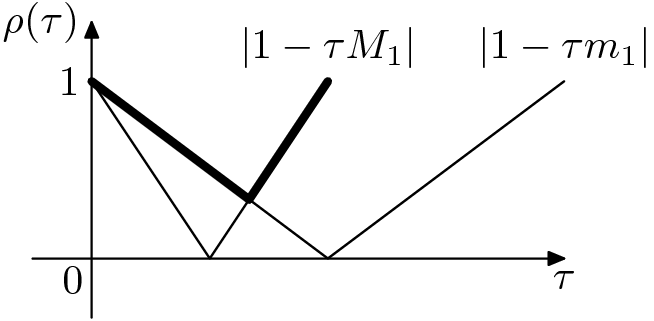
\includegraphics[width=.5\linewidth]{mal-1.png}
\end{figure}

% u:=1cm;
% label.llft(btex $0$ etex, (0,0));
% label.lft(btex $1$ etex, (0,3u/2));
% drawarrow (-u/2,0)--(4u,0);
% drawarrow (0,-u/2)--(0,2u);
% label.lft(btex $q(\tau)$ etex, (0,2u));
% label.bot(btex $\tau$ etex, (4u,0));
% draw (0,3u/2)--(u,0)--(2u,3u/2);
% draw (0,3u/2)--(2u,0)--(4u,3u/2);
% label.top(btex $|1-\tau \cdot M_1|$ etex, (2u,3u/2));
% label.top(btex $|1-\tau \cdot m_1|$ etex, (4u,3u/2));
% draw (4/3u,u/2)--(2u,3u/2) withpen pencircle scaled 2bp;
% draw (0,3u/2)--(4/3u,u/2) withpen pencircle scaled 2bp;
% label.bot(btex $\tau_0$ etex, (4/3u,0));

З графіка видно, що точка мінімуму визначається умовою $|1 - \tau \cdot M_1| = |1 - \tau \cdot m_1|$. \\

Тому
\[ 1 - \tau_0 \cdot m_1 = \tau_0 \cdot M_1 - 1 \Rightarrow \tau_0 = \dfrac{2}{M_1+m_1} < \dfrac{2}{|f'(x)|}.\]

При цьому значенні $\tau$ маємо \[q(\tau_0) = q_0 =\dfrac{M_1-m_1}{M_1+m_1}.\]

Тоді для похибки вірна оцінка \[|x_n-\overline{x}|\le \dfrac{q_0^n\cdot (b-a)}{1-q_0}<\epsilon.\]

Кількість ітерацій \[n = n(\epsilon) \ge \left\lfloor \dfrac{\ln \left(\dfrac{\epsilon\cdot(1-q_0)}{b-a}\right)}{\ln q_0} \right\rfloor + 1.\]	

\begin{problem} 
	Дати геометричну інтерпретацію методу простої ітерації для випадків:
	\[ 0 < \phi'(x) < 1; \quad -1 < \phi'(x) < 0; \quad \phi'(x) < -1; \quad \phi'(x) > 1,\]
\end{problem}

\begin{problem} 
	Знайти оптимальне $\tau = \tau_0$ для методу релаксації при $f'(x) > 0$.
\end{problem}

\subsection{Метод Ньютона (метод дотичних)}

Припустимо, що рівняння $f (x) = 0$ має простий дійсний корінь $\overline{x}$, тобто $f (\overline{x}) = 0$, $f'(\overline{x}) \ne 0$. Нехай виконуються умови: $f (x)\in C^{(1)}([a,b])$, $f (a)\cdot f (b) < 0$. Тоді 
\[0 = f (\overline{x}) = f (x_k + \overline{x} - x_k ) = f (x_k ) + f'(\xi_k ) \cdot (\overline{x} - x_k ),\] 
де $\xi_k=x_k+\theta_k \cdot (\overline{x}-x_k)$, $0 < \theta_k < 1$, $\xi_k \approx x_k$. Тому наступне наближення виберемо з рівняння 
\[ f(x_k) + f'(x_k) \cdot (x_{k+1}-x_k) = 0.\]

Звідси маємо ітераційний процес
\[ x_{k+1} = x_k - \dfrac{f(x_k)}{f'(x_k)}, \quad k = 0,1,2,\ldots, \quad x_0\text{ -- задане}. \]

Метод Ньютона ще називають методом лінеаризації або методом дотичних.

\begin{problem} 
	Дати геометричну інтерпретацію методу Ньютона.
\end{problem}

Метод Ньютона можна інтерпретувати як метод простої ітерації з \[ \phi(x) = x - \dfrac{f(x)}{f'(x)}, \quad \text{тобто} \quad \tau(x) = - \dfrac{1}{f'(x)}. \]

Тому 
\[ \phi'(x) = 1 - \dfrac{f'(x)\cdot f'(x)-f(x)\cdot f''(x)}{(f'(x))^2} = \dfrac{f(x)\cdot f''(x)}{(f'(x))^2}.\]
Якщо $\overline{x}$ -- корінь $f(x)$, то $\phi'(x) = 0$. Тому знайдеться окіл кореня, де \[ |\phi'(x)| = \left|\dfrac{f(x)\cdot f''(x)}{(f'(x))^2}\right|<1.\]

Це означає, що збіжність методу Ньютона залежить від вибору $x_0$. \\

Недолік методу Ньютона: необхідність обчислювати на кожній ітерації не тільки значення функції, а й похідної. \\

Модифікований метод Ньютона позбавлений цього недоліку і має вигляд:
\[ x_{k+1} = x_k - \dfrac{f(x_k)}{f'(x_0)}, \quad k=0,1,2,\ldots. \]

Цей метод має лише лінійну збіжність: $|x_{k+1} - \overline{x}| = O(|x_k-\overline{x}|)$.
\begin{problem} 
	Дати геометричну інтерпретацію модифікованого методу Ньютона.
\end{problem}

В методі Ньютона, для якого $f'(x_k)$ замінюється на $\frac{f(x_k)-f(x_{k-1})}{x_k-x_{k-1}}$ дає метод січних: \[ x_{k+1} = x_k - \dfrac{x_k-x_{k-1}}{f(x_k)-f(x_{k-1})}\cdot f(x_k), \quad k = 1,2,\ldots, \quad x_0,x_1\text{ -- задані}.\]

\begin{problem} 
	Дати геометричну інтерпретацію методу січних.
\end{problem}

\subsection{Збіжність методу Ньютона}

\begin{theorem}
	Нехай $f(x)\in C^{(2)}([a,b])$, $\overline{x}$ -- простий дійсний корінь рівняння
	\begin{equation}
		\label{eq:2.10}
		f (x) = 0
	\end{equation}
	і $f'(x) \ne 0$ при $x\in U_r= \{x: |x -\overline{x}| < r\}$. Якщо
	\begin{equation}
		\label{eq:2.11}
		\dfrac{M_2\cdot|x_0-\overline{x}|}{2m_1} = q < 1
	\end{equation}
	де $m_1 = \Min_{x\in U_r} |f'(x)|$, $M_2 = \Max_{x\in U_r} |f''(x)|$, то для $x_0 \in U_r$ метод Ньютона 
	\begin{equation}
		\label{eq:2.12}
		x_{k+1} = x_k - \dfrac{f(x_k)}{f'(x_k)}
	\end{equation}
	збігається і має місце оцінка
	\begin{equation}
		\label{eq:2.13}
		|x_n - \overline{x}| \le q^{2^n-1} \cdot |x_0 - \overline{x}|.
	\end{equation}
\end{theorem}

\begin{proof}
	З (\ref{eq:2.12}) маємо 
	\begin{equation}
		\label{eq:2.14}
		x_{k+1} - \overline{x} = x_k - \dfrac{f(x_k)}{f'(x_k)} - \overline{x} = \dfrac{(x_k-\overline{x}) \cdot f'(x_k)-f(x_k)}{f'(x_k)} = \dfrac{F(x_k)}{f'(x_k)},
	\end{equation}
	де $F(x) = (x - \overline{x}) \cdot f'(x) - f (x)$, така, що
	\begin{enumerate}
		\item $F(x) = 0$;
		\item $F'(x) = (x - \overline{x}) \cdot f''(x)$;
	\end{enumerate}
	Тоді \[ F(x_k) = F(\overline{x}) + \Int_{\overline{x}}^{x_k}  F'(t) \diff t = \Int_{\overline{x}}^{x_k}  ((t - \overline{x}) \cdot f''(t)) \diff t . \]

	Так як $(t - x)$ не міняє знак на відрізку інтегрування, то скористаємося теоремою про середнє значення:
	\begin{equation}
		\label{eq:2.15}
		F(x_k) = f''(\xi_k) \Int_{\overline{x}}^{x_k}  (t - \overline{x}) \diff t = \dfrac{(x_k-\overline{x})^2}{2} f''(\xi_k),
	\end{equation}
	де $\xi_k = \overline{x} + \theta_k \cdot (x_k - \overline{x})$, $0 <\theta_k < 1$. З (\ref{eq:2.14}), (\ref{eq:2.15}) маємо
	\begin{equation}
		\label{eq:2.16}
		x_{k+1} - \overline{x} = \dfrac{(x_k-\overline{x})^2}{2f'(x_k)} f''(\xi_k).
	\end{equation}
	Доведемо оцінку (\ref{eq:2.12}) за індукцією. Так як $x_0 \in U_r$, то \[|\xi_0 - \overline{x}| = |\theta_0 \cdot (x_0 - \overline{x})| < |\theta_0| \cdot |x_0 - \overline{x}| < r \Rightarrow \xi_0 \in U_r.\]

	Тоді $f''(\xi_0) \le M_2$, тому
	\begin{multline*} 
		|x_1 - \overline{x}| \le \dfrac{(x_0-\overline{x})^2 \cdot M_2}{2m_1} = \dfrac{M_2\cdot|x_0-\overline{x}|}{2m_1}|x_0-\overline{x}| = \\
		= q\cdot |x_0-\overline{x}|=q\cdot |x_0-\overline{x}|<r \Rightarrow x_1\in U_r.
	\end{multline*}

	Ми довели твердження (\ref{eq:2.13}) при $n = 1$. Нехай воно справджується при $n = k$:
	\[ |x_k - \overline{x}| \le q^{2^k-1}\cdot |x_0 - \overline{x}| < r, \quad |\xi_k - \overline{x}| = |\theta_k \cdot (x_k - \overline{x})| < r. \]

	Тоді $x_k, \xi_k \in U_r$. \\

	Доведемо (\ref{eq:2.13}) для $n = k +1$. З (\ref{eq:2.16}) маємо 
	\begin{multline*}
		|x_{k+1}-\overline{x}| \le \dfrac{|x_k - \overline{x}|^2\cdot M_2}{2m_1} \le \left(q^{2^k-1}\right)^2 \dfrac{|x_0-\overline{x}|^2\cdot M_2}{2m_1} = \\
		= q^{2^{k+1}-2} \dfrac{|x_0-\overline{x}|\cdot M_2}{2m_1}|x_0-\overline{x}| = q^{2^{k+1}-1} \cdot |x_0-\overline{x}|.
	\end{multline*}

	Таким чином (\ref{eq:2.13}) справджується для $n = k +1$. Значить (\ref{eq:2.13}) виконується і для довільного $n$. Таким чином $x_n \xrightarrow[n\to\infty]{} \overline{x}$.
\end{proof}

З (\ref{eq:2.13}) маємо оцінку кількості ітерацій для досягнення точності $\epsilon$:
\[ n \ge \left\lfloor\log_2\left(1+\dfrac{\ln \left(\dfrac{\epsilon}{b-a}\right)}{\ln q}\right) \right\rfloor + 1 .\]

Кажуть, що ітераційний метод має \textit{степінь збіжності} $m$, якщо \[ |x_{k+1}-\overline{x}|=O(|x_k-\overline{x}|^m).\]

Для методу Ньютона 
\[|x_{k+1}-\overline{x}| = \dfrac{|x_k-\overline{x}|^2\cdot|f''(\xi_k)|}{2|f'(x_k)|}| \Rightarrow |x_{k+1}-\overline{x}|=O(|x_k-\overline{x}|^2).\]

Значить степінь збіжності методу Ньютона $m=2$. Для методу простої ітерації і ділення навпіл $m=1$.

\begin{theorem}
	Нехай $f(x)\in C^{(2)}([a,b])$ та $\overline{x}$ -- простий корінь рівняння $f (x) = 0$ а також $\forall x\in[a,b]$: $f'(x) \ne 0$. Якщо $f'(x) \cdot f''(x) > 0$ ($f'(x) \cdot f''(x) < 0$) то для методу Ньютона при $x_0 = b$ послідовність наближень $\{x_k \}$ монотонно спадає (монотонно зростає при $x_0 = a$).
\end{theorem}

\begin{problem}
	Довести теорему при 
	\begin{enumerate}
		\item $f'(x) \cdot f''(x) > 0$;
		\item $f'(x) f''(x) < 0$.
	\end{enumerate}
\end{problem}

\begin{problem}
	Знайти степінь збіжності методу січних.
\end{problem}


Якщо $f(a) \cdot f''(a) > 0$ та $f''(x)$ не міняє знак, то потрібно вибирати $x_0 = a$; при цьому $\{x_k \}\uparrow \overline{x}$. \\

Якщо $f(b) \cdot f''(b) > 0$, то $x_0 = b$; маємо $\{x_k \}\downarrow \overline{x}$. Пояснення на рисунку:

% u := 1cm;
% drawarrow (-u/2, 0)--(4u, 0);
% drawarrow (0, -u/2)--(0, 2u);
% draw (u/2,0)--(u/2,u/8);
% draw (7u/2,0)--(7u/2,u/8);
% label.bot(btex $a$ etex, (u/2, 0));
% label.top(btex $b$ etex, (7u/2, u/8));
% draw (u/2,3u/2){dir -75}..(2u,-u/2){dir 0}..(7u/2,-u/4);
% label.top(btex $x_0 = a$ etex, (2u,u));

% u := 1cm;
% drawarrow (-u/2, 0)--(4u, 0);
% drawarrow (0, -u/2)--(0, 2u);
% draw (u/2,0)--(u/2,u/8);
% draw (7u/2,0)--(7u/2,u/8);
% label.top(btex $a$ etex, (u/2, u/8));
% label.bot(btex $b$ etex, (7u/2, 0));
% draw (u/2,-3u/7){dir 75}..(2u,u)..(7u/2,3u/2);
% label.top(btex $x_0 = a$ etex, (2u,3u/2));

\begin{figure}[H]
	\centering
	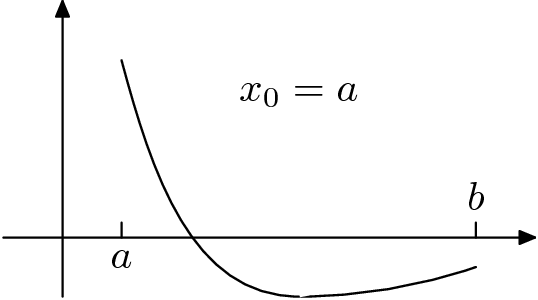
\includegraphics[width=.45\linewidth]{mal-2.png}
	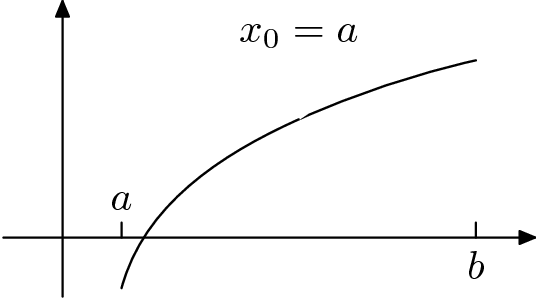
\includegraphics[width=.45\linewidth]{mal-3.png}
\end{figure}

\begin{remark}
	Якщо $\overline{x}$ -- $p$-кратний корінь тобто $f^{(m)} (x) = 0$, $m = \overline{0,p-1}$, $f^{ (p)} (x) \ne 0$, то в методі Ньютона необхідна наступна модифікація \[x_{k+1} = x_k - p\dfrac{f(x_k)}{f'(x_k)} \quad \text{і} \quad q = \dfrac{M_{p+1}\cdot|x_0-\overline{x}|}{m_p \cdot (p+1)}<1.\]
\end{remark}

\begin{remark}
Метод Ньютона можна застосовувати і для обчислення комплексного кореня, тоді ітераційний процес має вигляд \[z_{k+1} = z_k - \dfrac{f(z_k)}{f'(z_k)}, \quad k = 0,1,\ldots.\] В теоремі про збіжність $q = \frac{|z_0-\overline{z}|\cdot M_2}{2m_1}$, де $m_1 = \Min_{z\in U_r} |f'(z)|$, $M_2 = \Max_{z\in U_r} |f''(z)|$. Тут $|z|$ -- модуль комплексного числа $z$.
\end{remark}

Переваги методу Ньютона: 
\begin{enumerate}
\item висока швидкість збіжності;
\item узагальнюється на системи рівнянь; 
\item узагальнюється на комплексні корені.
\end{enumerate}
Недоліки методу Ньютона: 
\begin{enumerate}
	\item на кожній ітерації обчислюється не тільки $f (x_k )$ , а і похідна $f'(x_k)$;
	\item  збіжність залежить від початкового наближення $x_0$, так як від нього залежить умова збіжності $q = \frac{M_2\cdot |x_0-\overline{x}|}{2m_1} < 1$;
	\item потрібно, щоб $f (x)\in C^{(2)}([a,b])$.
\end{enumerate}

\section{Методи розв’язання СЛАР}

Методи розв’язування СЛАР поділяються на прямі та ітераційні. При умові точного виконання обчислень прямі методи за скінчену кількість операцій в результаті дають точний розв’язок. Використовуються вони для невеликих та середніх СЛАР $n=10^2..10^4$. Ітераційні методи використовуються для великих СЛАР $n>10^5$, як правило розріджених. В результаті отримуємо
послідовність наближень, яка збігається до розв’язку. \\

\subsection{Метод Гаусса}

Розглянемо задачу розв'язання СЛАР
\begin{equation}
	\label{eq:3.1}
	A \vec x = \vec b,
\end{equation}
причому $A = (a_{i,j})_{i,j=1}^n$, $\det A \ne 0$, $\vec x = (x_i)_{i=1}^n$, $\vec b = (b_j)_{j=1}^n$. Метод Крамера з обчисленням визначників для такої системи має складність $Q = O(n! n)$. \\

Запишемо СЛАР у вигляді
\begin{equation}
	\label{eq:3.2}
	\left\{
		\begin{matrix}
			a_{1,1} x_1 + a_{1,2} x_2 + \ldots + a_{1,n} x_n = b_1 \equiv a_{1,n+1} \\
			a_{2,1} x_1 + a_{2,2} x_2 + \ldots + a_{2,n} x_n = b_1 \equiv a_{2,n+1} \\
			\ldots \\
			a_{n,1} x_1 + a_{n,2} x_2 + \ldots + a_{n,n} x_n = b_1 \equiv a_{n,n+1}
		\end{matrix}
	\right.
\end{equation}

Якщо $a_{1,1} \ne 0$, то ділимо перше рівняння на нього і виключаємо $x_1$ з інших рівнянь: 

\[\left\{
	\begin{aligned}
		x_1 + a_{1,2}^{(1)} x_2 + \ldots + a_{1,n}^{(1)} x_n = a_{1,n+1}^{(1)} &\\
		a_{2,2}^{(1)} x_2 + \ldots + a_{2,n}^{(1)} x_n = a_{2,n+1}^{(1)} &\\
		\ldots &\\
		a_{n,2}^{(1)} x_2 + \ldots + a_{n,n}^{(1)} x_n = a_{n,n+1}^{(1)}&
	\end{aligned}
\right.\]

Процес повторюємо для $x_2, \ldots, x_n$. В результаті отримуємо систему з трикутною матрицею
\begin{equation}
	\label{eq:3.3}
	\left\{
		\begin{aligned}
		x_1 + a_{1,2}^{(1)} x_2 + \ldots + a_{1,n}^{(1)} x_n = a_{1,n+1}^{(1)}& \\
		x_2 + \ldots + a_{2,n}^{(2)} x_n = a_{2,n+1}^{(2)}& \\
		\ldots & \\
		x_n = a_{n,n+1}^{(n)} &
	\end{aligned}
	\right.
\end{equation}

Це прямий хід методу Гаусса. Формули прямого ходу
\[
	\left\{
		\begin{aligned}
			& k = \overline{1, n-1}: \\
			& a_{k,j}^{(k)} = \dfrac{a_{k,j}^{(k-1)}}{a_{k,k}^{(k-1)}}, \quad j =\overline{k+1,n+1}, \\
			& a_{i,j}^{(k)} = a_{i,j}^{(k-1)} - a_{i,k}^{(k-1)} a_{k,j}^{(k)}, \\
			& i = \overline{k+1, n}, \quad j = \overline{k +1, n + 1}.
		\end{aligned}
	\right.
\]
Звідси
\begin{equation}
	\label{eq:3.4}
	x_n = a_{n,n+1}^{(n)}, \quad x_i = a_{i,n+1}^{(i)} - \Sum_{j=i+1}^n a_{i,j}^{(i)} x_j, \quad i = \overline{n-1,1}.
\end{equation}

Це формули оберненого ходу. \\

Складність, тобто кількість операцій, яку необхідно виконати для реалізації методу, -- $Q_{\text{np}} = \frac23 n^3 + O(n^2)$ для прямого ходу, $Q_{\text{об}} = n^2 + O(n)$ для оберненого ходу. \\

Умова $a_{k,k}^{(k-1)} \ne 0$ не суттєва, оскільки знайдеться $m$, для якого $|a_{m,k}^{(k-1)}| = \Max_i |a_{i,k}^{(k-1)}| \ne 0$ (оскільки $\det A \ne 0$). Тоді міняємо місцями рядки номерів $k$ і $m$ . Елемент $a_{k,k}^{(k-1)} \ne 0$ називається ведучим. \\

Введемо матриці \[ M_k = \begin{pmatrix} 1 & & & & 0 \\ & \ddots & & & \\ 0 & & m_{k,k} & & \\ & & \vdots & \ddots & \\0 & & m_{n,k} & & 1 \end{pmatrix},\]
елементи якої обчислюється так $m_{k,k} = \dfrac{1}{a_{k,k}^{(k-1)}}$, $m_{k,k}=-\dfrac{a_{i,k}^{(k-1)}}{a_{k,k}^{(k-1)}}$. \\

Нехай на $k$-му кроці $A_{k-1}\vec x = \vec b_{k-1}$. Множимо цю СЛАР зліва на $M_k$: $M_k A_{k-1}\vec x = M_k \vec b_{k-1}$. Позначимо $A_k = M_k A_{k-1}$; $A_0 = A$. Тоді прямий хід методу Гаусса можна записати у вигляді \[ M_n M_{n-1} \ldots M_1 A \vec x = M_n M_{n-1} \ldots M_1 \vec b.\]

Позначимо останню систему, яка співпадає з (\ref{eq:3.2}), так 
\begin{equation}
	\label{eq:3.5}
	U \vec x = \vec c, \quad U = (u_{i,j})_{i,j=1}^n,
\end{equation}
причому \[ \left\{ \begin{aligned} & u_{i,i} = 1 \\ & u_{i,j} = 0, \quad i > j \end{aligned} \right.\]

Таким чином $U = M_n M_{n-1} \ldots M_1 A$. Введемо матриці
\[ L_k = \begin{pmatrix} 1 & & 0 & & 0 \\ & \ddots & & & \\ 0 & & a_{k,k}^{(k-1)} & & 0 \\ & & \vdots & \ddots & \\0 & & a_{n,k}^{(k-1)} & & 1 \end{pmatrix},\]

Тоді \[A = L_1\ldots L_n U = LU; \quad  L = L_1\ldots L_n, \]
$L$ -- нижня трикутня матриця, $U$ -- верхня трикутня матриця. Таким чином метод Гаусса можна трактувати, як розклад матриці $А$ в добуток двох трикутних матриць -- ($LU$)-розклад. \\

Введемо матрицю $P_k$ перестановок на $k$-му кроці (це матриця, отримана з одиничної матриці перестановкою $k$-того і $m$-того рядка). Тоді при множені на неї матриці $A_{k-1}$ робимо ведучим елементом максимальний за модулем. \\ % P_k ? 

За допомогою цих матриць перехід до трикутної системи (\ref{eq:3.3-1}) тепер має вигляд: \[ M_n M_{n-1} P_{n-1} \ldots M_1 P_1 A \vec x = M_n M_{n-1} P_{n-1} \ldots M_1 P_1 \vec b. \]

\textbf{Твердження}: знайдеться така матриця $Р$ -- перестановок, що $PA = LU$ -- розклад матриці на нижню трикутну з ненульовими діагональними елементами і верхню трикутну матрицю з одиницями на діагоналі. \\

\textbf{Висновки про переваги трикутного розкладу}:
\begin{enumerate}
	\item Розділення прямого і оберненого ходів дає змогу економно розв'язувати декілька систем з одноковою матрицею та різними правими частинами.
	\item Зберігання $M$, або $L$ та $U$ на місці $A$.
	\item Обчислюючи $l$ -- кількість перестановок, можна встановити знак визначника.
\end{enumerate}

\subsection{Метод квадратних коренів}
Цей метод призначений для розв'язання систем рівнянь із симетричною матрицею
\begin{equation}
	\label{eq:3.6}
	A \vec x = \vec b, \quad A^T = A.
\end{equation}
Він оснований на розкладі матриці $A$ в добуток:
\begin{equation}
	\label{eq:3.7}
	A = S^T D S,
\end{equation}
$S$ -- верхня трикутна матриця, $S^T$ -- нижня трикутна матриця, $D$ -- діагональна матриця. \\

Виникає питання: як обчислити $S$, $D$ по матриці $A$? Маємо
\begin{equation}
	\label{eq:3.8}
	\begin{aligned}
		& (DS)_{i,j} = \begin{cases} d_{i,i}s_{i,j}, & i \le j \\ 0, & i > j \end{cases} \\
		& (S^TDS)_{i,j} = \Sum_{l=1}^n s_{i,l}^T d_{l,l} s_{l, j} = \Sum_{l=1}^{i-1} s_{l,i} s_{l, j} d_{l, l} + s_{i,i} s_{i,j} d_{i,i} + \\
		& +\underset{=0}{\underbrace{\Sum_{l=i+1}^n s_{l, i} s_{l, j} s_{l,l}}} = a_{i,j}, \quad i,i = \overline{1,n}. 
	\end{aligned}
\end{equation}
Якщо $i = j$, то \[ |s_{i,i}^2|d_{i,i} = a_{i,i} - \Sum_{l=1}^{i-1} |s_{l,i}^2| d_{l,l] \equiv p_i}.\]

Тому \[ d_{i,i} = sign (p_i), \quad s_{i,i} = \sqrt{|p_i|}. \]

Якщо $i < j$, то \[ s_{i,j} = \left( a_{i,j} - \Sum_{l=1}^{i-1} s_{l,i} d_{l,l} s_{l,j} \right) / (s_{i,i} d_{i,i}), \quad i = \overline{1, n}, \quad j = \overline{i+1, n}. \]

Якщо $A > 0$ (тобто головні мінори матриці $A$ додатні), то всі $d_{i,i} = +1$. \\

Знайдемо розв’язок рівняння (\ref{eq:3.2.1}). Враховуючи (\ref{eq:3.2.2}), маємо:
\begin{equation}
	\label{eq:3.9}
	S^T D \vec y = \vec b
\end{equation}
\begin{equation}
	\label{eq:3.10}
	S \vec x = \vec y
\end{equation}
Оскільки $S$ -- верхня трикутна матриця, а $S^TD$ -- нижня трикутна матриця, то
\begin{equation}
	\label{eq:3.11}
	y_i = \dfrac{b_i - \Sum_{j=1}^{i-1} s_{j,i}s_{j,j}y_j}{s_{i,i}d_{i,i}}, \quad i=\overline{1,n}
\end{equation}
\begin{equation}
	\label{eq:3.12}
	x_n = \dfrac{y_n}{s_{n,n}}, \quad x_i = \dfrac{y_i - \Sum_{j=1}^{i-1} s_{i,j} x_j}{s_{i,i}}, \quad i=\overline{n-1,1}.
\end{equation}

Метод застосовується лише для симетричних матриць. Його складність -- $Q = \frac13 n^3 + O(n^2)$. \\

Переваги цього методу:
\begin{enumerate}
	\item він витрачає в 2 рази менше пам'яті ніж метод Гаусса для зберігання $A^T = A$ (необхідний об'єм пам'яті $\dfrac{n(n+1)}{2} \sim \dfrac{n^2}{2}$;
	\item метод однорідний, без перестановок;
	\item якщо матриця $A$ має багато нульових елементів, то і матриця $S$ також.
\end{enumerate}
Остання властивість дає економію в пам'яті та кількості арифметичних операцій. Наприклад, якщо $A$ має $m$ ненульових стрічок по діагоналі, то $Q = O(m^2n)$.

\subsection{Обчислення визначника та оберненої матриці}

Кількість операцій обчислення детермінанту за означенням -- $Q_{\det} = n!$. В методі Гаусса -- $PA = LU$. Тому 
\begin{equation}
	\label{eq:3.13} 
	\det P \det A = \det L \det U \Rightarrow \det A = (-1)^l \det L \det U = (-1)^l \Prod_{k=1}^n a_{k,k}^{(k)},
\end{equation}
де $l$ -- кількість перестановок. Ясно, що за методом Гаусса \[Q_{\det} = \dfrac 23 n^3 + O (n^2) .\]

В методі квадратного кореня $A = S^T D S$. Тому 
\begin{equation}
	\label{eq:3.14}
	\det A = \det S^T \det D \det S = \Prod_{k=1}^n d_{k,k} \Prod_{k=1}^n s_{k,k}^2.
\end{equation}

Тепер $Q_{\det} = \frac 13 n^3 + O(n^2)$. \\

За означенням 
\begin{equation}
	\label{eq:3.15}
	AA^{-1} = E
\end{equation}
де $A^{-1}$ обернена до матриці $A$. Позначимо
\[ A^{-1} = (\alpha_{i,j})_{i,j=1}^n.\] 

Тоді $\vec \alpha_j = (\alpha_{i,j})_{i=1}^n$ -- вектор-стовпчик оберненої матриці. З (\ref{eq:3.15}) маємо
\begin{equation}
	\label{eq:3.16}
	A \vec \alpha_j = \vec e_j, \quad j = \overline{1, n},
\end{equation}
$\vec e_j$ -- стовпчики одиничної матриці: $\vec e_j = (\delta_{i,j})_{i=1}^n$, $\delta_{i,j} = \begin{cases} 1, & i = j \\ 0, & i \ne j \end{cases}$. \\

Для знаходження $А^{-1}$ необхідно розв'язати $n$ систем. Для знаходження $A^{-1}$ методом Гаусса необхідна кількість операцій $Q = 2n^3 + O(n^2)$.

\subsection{Метод прогонки}

Це економний метод для розв'язання СЛАР з три діагональною матрицею:
\begin{equation}
	\label{eq:3.17}
	-c_0 y_0 + b_0 y_1 = - f_0,
\end{equation}
\begin{equation}
	\label{eq:3.18}
	a_i y_{i-1} - c_i y_i + b_i y_{i+1} = -f_i,
\end{equation}
\begin{equation}
	\label{eq:3.19}
	a_N y_{N-1} - c_N y_N = -f_N.
\end{equation}
Матриця системи
\[ A = \begin{pmatrix} -c_0 & b_1 & & 0 \\ a_0 & -c_11 & \ddots & \\ & \ddots & \ddots & b_N \\ 0 & & a_N & -c_N \end{pmatrix}\]
тридіагональна. \\

Розв'язок представимо у вигляді
\begin{equation}
	\label{eq:3.20}
	y_i = \alpha_{i+1} y_{i+1} + \beta_{i+1}, \quad i = \overline{0, N-1}.
\end{equation}
Замінимо в (\ref{eq:3.20}) $i \mapsto i-1$ і підставимо в (\ref{eq:3.18}), тоді \[ (a_i \alpha_i - c_i) y_i + b_i y_{i+1} = - f_i - a_i \beta_i. \]

Звідси \[ y_i = \dfrac{b_i}{c_i - a_i\alpha_i} y_{i+1} + \dfrac{f_i + a_i \beta_i}{c_i - a_i \alpha_i}.\]

Тому з (\ref{eq:3.18}) \[ \alpha_{i+1} = \dfrac{b_i}{c_i - a_i\alpha_i}, \quad \beta_{i+1} = \dfrac{f_i+a_i\beta_i}{c_i-a_i\alpha_i}, \quad i=\overline{1, N-1}.\]

Умова розв'язності (\ref{eq:3.17}) $c_i - a_i \alpha_i \ne 0$. \\

Щоб знайти всі $\alpha_i$, $\beta_i$, треба задати перші значення. З (\ref{eq:3.17}):
\begin{equation}
	\label{eq:3.21}
	\alpha_1 = \dfrac{b_0}{c_0}, \quad \beta_1 = \dfrac{f_0}{c_0}.
\end{equation}
Після знаходження всіх $\alpha_i$, $\beta_i$ обчислюємо $y_N$ з системи
\[ \left\{ \begin{aligned} & a_N y_N - c_n y_N = - f_N, \\ & y_{N-1} = \alpha_N y_N + \beta_N \end{aligned} \right. \]

Звідси
\begin{equation}
	\label{eq:3.22}
	y_N = \dfrac{f_N + a_n \beta_N}{c_N - a_N \alpha_N}.
\end{equation}

\textbf{Алгоритм}
\begin{enumerate}
	\item Покладемо $\alpha_1 = \frac{b_0}{c_0}$, $\beta_1 = \frac{f_0}{c_0}$.

	\item Позначимо $z_i = c_i - a_i \alpha_i$, обчислимо $\alpha_{i+1} = \frac{b_i}{z_i}$, $\beta_{i+1} = \frac{f_i+a_i\beta_i}{z_i}$, для $i=\overline{1,N-1}$.

	\item Знайдемо $y_N = \frac{f_N + a_N \beta_N}{c_N - a_N \alpha_N}$.

	\item Обчислюємо $y_i = \alpha_{i+1} y_{i+1} + \beta_{i+1}$, $i=\overline{N-1,0}$.
\end{enumerate}
Складність алгоритму $Q = 8N - 2$. \\

Метод можна застосовувати, коли $\forall i$: $c_i - a_i \alpha_i \ne 0$, $|\alpha_i| \le 1$. Якщо $|\alpha_i| \ge q > 1$, то $\Delta y_0 \ge q^N \Delta y_N$ (тут $\Delta y_i$ абсолютна похибка обчислення $y_i$), а це приводить до експоненціального накопичення похибок заокруглення, тобто нестійкості алгоритму прогонки.

\begin{theorem}[про достатні умови стійкості метода прогонки]
Нехай \[ \forall i: a_i, b_i \ne 0, \quad \text{та} \quad |c_i| \ge |a_i| + |b_i| \quad (a_0 = b_N = 0),\] та хоча би одна нерівність строга. Тоді \[ |\alpha_i| \le 1, \quad \text{та} \quad z_i = c_i - a_i \alpha_i \ne 0, \quad i = \overline{1,N}.\]
\end{theorem}

\begin{problem}
	Довести теорему про стійкість методу прогонки.
\end{problem}

\subsection{Обумовленість систем лінійних алгебраїчних рівнянь}

Нехай задано СЛАР
\begin{equation}
	\label{eq:3.23}
	A \vec x = \vec b.
\end{equation}

Припустимо, що матриця і права частина системи задані неточно і фактично розв'язуємо систему
\begin{equation}
	\label{eq:3.24}
	B \vec y = \vec h.
\end{equation}
де $B = A + C$, $\vec h = \vec b + \vec \eta$, $\vec y = \vec x + \vec z$. \\

Малість детермінанту $\det A \ll 1$ не є необхідною умовою різкого збільшення похибки. Це ілюструє наступний приклад: \[A = diag(\epsilon), \quad a_{i,j} = \epsilon \Delta_{i,j}.\]

Тоді $\det A = \epsilon^n \ll 1$, але $x_i = \frac{b_i}{\epsilon}$. Тому $\Delta x_i = \frac{\Delta b_i}{\epsilon}$. \\

Оцінимо похибку розв’язку. Підставивши значення $B$, $\vec h$, та $\vec z = \vec y - \vec x$, отримаємо: \[ (A+C)(\vec x + \vec z) = \vec b +\vec \eta.\]

Віднімемо від цієї рівності (\ref{eq:3.5.1}) $A \vec z + C \vec x + C \vec z = \vec \eta$. Тоді
\[ A \vec z = \vec \eta - C \vec x - C \vec z, \quad \vec z = A^{-1}(\vec \eta - C \vec x - C \vec z).\]

Введемо норми векторів: $\|\vec z\|$:
\[ \|\vec z\|_1 = \Sum_{i=1}^n |z_i|, \quad \|\vec z\|_2 = \left(\Sum_{i=1}^n |z_i|^2\right)^{1/2}, \quad \|\vec z\|_\infty = \Max_i |z_i|. \]

Норми матриці, що відповідають нормам вектора, тобто
\[ \|A\|_m = \Sup_{\|\vec x\|_m \ne 0} \dfrac{\|A\vec x\|_m}{\|\vec x\|_m}, \quad m=1,2,\infty. \]
такі: \[ \|A\|_1 = \Max_j \Sum_{i=1}^n |a_{i,j}|, \quad \|A\|_2 = \Max_i \sqrt{\lambda_i (A^TA)}, \quad \|A\|_\infty = \Max_i \Sum_{j=1}^n |a_{i,j}|, \]
де $\lambda_i(B)$ -- власні значення матриці $B$. \\

Позначимо $\delta(\vec x) = \frac{\|\vec z\|}{\|\vec x\|}$, $\delta(\vec b) = \frac{\|\vec \eta\|}{\|\vec b\|}$, $\delta(A) = \frac{\|C\|}{\|A\|}$ -- відносні похибки $\vec x$, $\vec b$, $A$, де $\|\cdot\|_k$ -- одна з введених вище норм. \\

Для характеристики зв'язку між похибками правої частини та розв'язку вводять поняття обумовленості матриці системи. \\

\textit{Число обумовленості матриці} $A$ -- $\cond (A) = \|A\|\|A^{-1}\|$.

\begin{theorem}
	Якщо $\exists A^{-1}$ та $\|A^{-1}\|\|C\|<1$, то
	\begin{equation}
		\label{eq:3.25}
		\delta(\vec x) \le \dfrac{\cond (A)}{1-\cond (A)\delta(A)}(\delta(A)+\delta(\vec b)),
	\end{equation}
	де $\cond (A)$ -- число обумовленості.
\end{theorem}
\begin{proof}
	\[A \vec z = \vec \eta - C \vec x - C \vec z, \quad \vec z = A^{-1} \vec \eta - A^{-1} C \vec x - A^{-1} C \vec z\]
	\[ \|\vec z\| \le \|A^{-1}\vec \eta\|+\|A^{-1}C\vec x\| +\|A^{-1}C\vec z\| \le \|A^{-1}\|\cdot\|\vec \eta\|+\|A^{-1}\|\cdot \|C\|\cdot \|\vec x\| +\|A^{-1}\|\cdot \|C\|\cdot \|\vec z\|. \]
	\[ \|\vec z\| \le \dfrac{\|A^{-1}\|(\|\vec\eta\|+\|C\|\cdot\|\vec x\|)}{1 - \|A^{-1}\| \cdot \|C\|} \]

	Оцінка похибки
	\begin{multline*}
		\delta(\vec x) \le \dfrac{\|A^{-1}\|}{1-\|A^{-1}\| \cdot \|C\|} \left(\dfrac{\|\vec \eta\|}{\|\vec x\|}+\|C\| \right) = \\
		= \dfrac{\|A^{-1}\|\cdot \|A\|}{1-\|A^{-1}\|\cdot\|A\|\cdot \dfrac{\|C\|}{\|A\|}} \left(\dfrac{\|\vec \eta\|}{\|A\|\cdot \|\vec x\|} + \delta(A) \right) \le \\
		\le \dfrac{\cond (A)}{1-\cond (A)\delta(A)}\left(\dfrac{\|\vec\eta\|}{\|\vec x\|}+\delta(A)\right).
	\end{multline*}
\end{proof}

\textbf{Наслідок}. Якщо $C \equiv 0$, то $\delta(\vec x) \le \cond  (A) \delta (\vec b)$. \\

\textbf{Властивості} $\cond (A)$:
\begin{enumerate}
	\item $\cond (A)\ge1$;
	\item $\cond (A)\ge\dfrac{\Max_i |\lambda_i(A)|}{\Min_i|\lambda_i(A)|}$;
	\item $\cond (AB) \le \cond (A) \cdot \cond (B)$;
	\item $A^T = A^{-1} \Rightarrow \cond (A) = 1$.
\end{enumerate}

Друга властивість має місце оскільки довільна норма матриці не менше її найбільшого за модулем власного значення. Значить $\|A\|\ge\max|\lambda_A|$. Оскільки власні значення матриць $A^{-1}$ та $A$ взаємно обернені, то \[ \|A^{-1}\| \ge \max \dfrac{1}{|\lambda_A|} = \dfrac{1}{\min|\lambda_A|}.\]

Якщо $1\ll \cond (A)$, то система називається \textit{погано обумовленою}. \\

Оцінка впливу похибок заокруглення при обчисленні розв‘язку СЛАР така (Дж. Уілкінсон): $\delta (A) = O(n\beta^{-t})$, $\delta(\vec b) = O(\beta^{-t})$, де $\beta$ -- розрядність ЕОМ, $t$ -- кількість розрядів, що відводиться під мантису числа. З оцінки (\ref{eq:3.5.3}) витікає: $\delta(\vec x) = \cond (A)\times O(n\beta^{-t})$. Висновок: найпростіший спосіб підвищити точність обчислення розв‘язку погано обумовленої СЛАР -- збільшити розрядність ЕОМ при обчисленнях. Інші способи пов'язані з розглядом цієї СЛАР як некоректної задачі із застосуванням відповідних методів її розв'язання. \\

Приклад погано обумовленої системи -- системи з матрицею Гільберта  \[ H_n = \left(\dfrac{1}{i+j-1}\right)_{i,j=1}^n, \quad \text{наприклад }\cond (H_8)\approx 10^9.\]


\section{Ітераційні методи для систем}

\subsection{Ітераційні методи розв'язання СЛАР}

Систему
\begin{equation}
	\label{eq:4.1}
	A \vec x = \vec b
\end{equation}
зводимо до вигляду
\begin{equation}
	\label{eq:4.2}
	\vec x = B \vec x + \vec f.
\end{equation}
Будь яка система
\begin{equation}
	\label{eq:4.3}
	\vec x = \vec x - C \cdot (A \vec x - \vec b)
\end{equation}
має вигляд (\ref{eq:4.2}) і при $\det C \ne 0$ еквівалентна системі (\ref{eq:4.1}). Наприклад, для $C = \tau \cdot E$:
\begin{equation}
	\label{eq:4.4}
	\vec x = \vec x - \tau \cdot (A \vec x - \vec b).
\end{equation}


\subsubsection{Метод простої ітерації}

Цей метод застосовується до рівняння (\ref{eq:4.2})
\begin{equation}
	\label{eq:4.5}
	\vec x^{(k+1)} = B \vec x^{(k)} + \vec f,
\end{equation}
де $\vec x^{(0)}$ -- початкове наближення, задано.\\

Ітераційний процес збігається, тобто $\left\| \vec x^{(k)} - \vec x\right\| \xrightarrow[k\to\infty]{} 0$, якщо
\begin{equation}
	\label{eq:4.6}
	\|B\| \le q < 1
\end{equation}
При цьому має місце оцінка
\begin{equation}
	\label{eq:4.7}
	\left\|\vec x^{(n)} - \vec x\right\| \le \dfrac{q^n}{1-q}\cdot\left\|\vec x^{(1)} - \vec x^{(0)}\right\|.
\end{equation}

\subsubsection{Метод Якобі}

Припустимо $\forall i$: $a_{i,i} \ne 0$. Зведемо систему (\ref{eq:4.1}) до вигляду
\[ x_i = -\Sum_{j=1}^{i-1} \dfrac{a_{i,j}}{a_{i,i}} \cdot x_j - \Sum_{j=i+1}^n \dfrac{a_{i,j}}{a_{i,i}} \cdot x_j + \dfrac{b_i}{a_{i,i}}, \quad i=\overline{1,n}. \]

Ітераційний процес запишемо у вигляді
\begin{equation}
	\label{eq:4.8}
	x_i^{(k+1)} = -\Sum_{j=1}^{i-1} \dfrac{a_{i,j}}{a_{i,i}} \cdot x_j^{(k)} - \Sum_{j=i+1}^n \dfrac{a_{i,j}}{a_{i,i}} \cdot x_j^{(k)} + \dfrac{b_i}{a_{i,i}}, \quad k = 0,1,\ldots, \quad i=\overline{1,n}.
\end{equation}

Ітераційний процес збігається до розв’язку, якщо виконується умова
\[ \forall i: \Sum_{\substack{j = 1 \\ i \ne j}}^n |a_{i,j}| \le |a_{i,i}|. \]

Це умова діагональної переваги матриці $A$. Якщо ж
\begin{equation}
	\label{eq:4.9}
	\forall i: \Sum_{\substack{j = 1 \\ i \ne j}}^n |a_{i,j}| \le q\cdot|a_{i,i}|, \quad 0 \le q < 1.
\end{equation}
то має місце оцінка точності:
\[ \|\vec x^{(n)} - \vec x\| \le \dfrac{q^n}{1-q}\cdot\|\vec x^{(0)}-\vec x\|. \]

\subsubsection{Метод Зейделя}
В компонентному вигляді ітераційний метод Зейделя записується так:
\begin{equation}
	\label{eq:4.10}
	x_i^{(k+1)} = -\Sum_{j=1}^{i-1} \dfrac{a_{i,j}}{a_{i,i}} \cdot x_j^{(k+1)} - \Sum_{j=i+1}^n \dfrac{a_{i,j}}{a_{i,i}} \cdot x_j^{(k)} + \dfrac{b_i}{a_{i,i}}, \quad k = 0,1,\ldots, \quad i=\overline{1,n}.
\end{equation}

На відміну від методу Якобі на $k$-му-кроці попередні компоненти розв'язку беруться з $k+1$-ої ітерації. \\

Достатня умова збіжності методу Зейделя -- $A^T = A > 0$.

\subsubsection{Матрична інтерпретація методів Якобі і Зейделя}

Подамо матрицю $A$ у вигляді \[ A = A_1 + D + A_2, \]
де $A_1$ -- нижній трикутник матриці $A$, $A_2$ -- верхній трикутник матриці $A$, $D$ -- її
діагональ. Тоді систему (\ref{eq:4.1}) запишемо у вигляді \[ D \vec x = A_1 \vec x + A_2 \vec x + \vec b,\]
або
\[ \vec x = D^{-1} A_1 \vec x + D^{-1} A_2 \vec x + D^{-1} \vec b,\]
 
Матричний запис методу Якобі:
\[ \vec x^{(k+1)} = D^{-1} A_1 \vec x^{(k)} + D^{-1} A_2 \vec x^{(k)} + D^{-1} \vec b,\]
методу Зейделя:
\[ \vec x^{(k+1)} = D^{-1} A_1 \vec x^{(k+1)} + D^{-1} A_2 \vec x^{(k)} + D^{-1} \vec b,\]

Необхідна і достатня умова збіжності методу Якобі: всі корені рівняння \[\det(D + \lambda(A_1 + A_2 )) = 0\] по модулю більше 1. \\

Необхідна і достатня умова збіжності методу Зейделя: всі корені рівняння \[\det(A_1 + D + \lambda A_2) = 0\] по модулю більше 1.

\subsubsection{Однокрокові (двошарові) ітераційні методи}

Канонічною формою однокрокового ітераційного методу розв'язку СЛАР є його запис у вигляді
\begin{equation}
	\label{eq:4.11}
	B_k \dfrac{\vec x^{(k+1)} - \vec x^{(k)}}{\tau_{k+1}} + A \vec x^{(k)} = \vec b,
\end{equation}

Тут $\{B_k\}$ -- послідовність матриць (пере-обумовлюючі матриці), що задають ітераційний метод на кожному кроці; $\{\tau_{k+1}\}$ -- ітераційні параметри. \\

Якщо $B_k = E$, то ітераційний процес називається \textit{явним}
\[ \vec x^{(k+1)} = \vec x^{(k)} - \tau_{k+1} \left(A \vec x^{(k)} + \vec b\right). \]
Якщо $B_k \ne E$, то ітераційний процес називається \textit{неявним}
\[ B_k \vec x^{(k+1)} = F^k. \]

У цьому випадку на кожній ітерації необхідно розв'язувати СЛАР. \\

Якщо $\tau_{k+1} \equiv \tau$, $B_k \equiv B$, то ітераційний процес називається \textit{стаціонарним}; інакше -- \textit{нестаціонарним}. \\

Методам, що розглянуті вище відповідають:
\begin{itemize}
	\item методу простої ітерації: $B_k = E$, $\tau_{k+1} = \tau$;
	\item методу Якобі: $B_k = D$, $\tau_{k+1} = 1$.;
	\item методу Зейделя: $B_k = D + A_1$, $\tau_{k+1} = 1$.
\end{itemize}

\subsubsection{Збіжності стаціонарних ітераційних процесів у випадку симетричних матриць}

Розглянемо випадок симетричних матриць $A^T=A$ і стаціонарний ітераційний процес $B_k \equiv E$, $\tau_{k+1} \equiv \tau$. \\

Нехай для $A$ справедливі нерівності
\begin{equation}
	\label{eq:4.12}
	\gamma_1 E \le A \le \gamma_2 E, \quad \gamma_1, \gamma_2 > 0.
\end{equation}

Тоді при виборі $\tau = \tau_0 = \frac{2}{\gamma_1 + \gamma_2}$ ітераційний процес збігається. Найбільш точним значенням $\gamma_1$, $\gamma_2$ при яких виконуються обмеження (\ref{eq:4.12}) є $\gamma_1 = \min \lambda_i(A)$, $\gamma_2 = \max \lambda_i(A)$. Тоді 
\[q = q_0 = \dfrac{\gamma_2 - \gamma_1}{\gamma_2 + \gamma_1} = \dfrac{1-\xi}{1+\xi}, \quad \xi = \dfrac{\gamma_1}{\gamma_2}.\]
(Зауважимо, що аналогічно обчислюється $q$ і для методу релаксації розв'язання нелінійних рівнянь, де $\gamma_1 = m = \min |f'(x)|$, $\gamma_2 = M_1 = \max|f'(x)|$) і справедлива оцінка\[ \|\vec x^{(n)} - \vec x\| \le \dfrac{q^n}{1-q} \cdot \|\vec x^{(0)} - \vec x\|. \]

Явний метод з багатьма параметрами $\{\tau_k\}$:
\[ B \equiv E, \quad \{\tau_k\}: \Min_\tau q(\tau), \quad n=n(\epsilon)\to\min,\]
які обчислюються за допомогою нулів багаточлена Чебишова, називаються ітераційним методом з чебишевським набором параметрів.

\subsubsection{Метод верхньої релаксації}

Узагальненням методу Зейделя є метод верхньої релаксації: \[ (D + \omega A_1) \cdot\dfrac{\vec x^{(k+1)} + \vec x^{(k)}}{\omega} + A \vec x^{(k)} = \vec b,\]
де $D$ -- діагональна матриця з елементами $a_{i,i}$ по діагоналі. $\omega > 0$ -- заданий числовий параметр. \\

Тепер $B = D + \omega A_1$, $\tau = \omega$. Якщо $A^T = A > 0$, то метод верхньої релаксації збігається при умові $0 < \omega < 2$. Параметр підбирається експериментально з умови мінімальної кількості ітерацій. 

\subsubsection{Методи варіаційного типу}

До цих методів відносяться: метод мінімальних нев’язок, метод мінімальних поправок, метод найшвидшого спуску, метод спряжених градієнтів. Вони дозволяють обчислювати наближення без використання апріорної інформації про $\gamma_1$, $\gamma_2$ в (\ref{eq:4.12}). \\

Нехай $B = E$. Для методу мінімальних нев’язок параметри $\tau_{k+1}$ обчислюються з умови 
\[ \left\|\vec r^{(k+1)}\right\|^2 = \left\|\vec r^{(k)}\right\|^2 - 2\tau_{k+1}\cdot\left(\vec r^{(k)}, A\vec r^{(k)}\right) + \tau_{k+1}^2 \cdot\left\|A\vec r^{(k)}\right|^2 \to \min. \]

Тому \[ \tau_{k+1} = \dfrac{\left(A\vec r^{(k)}, \vec r^{(k)}\right) }{\left\|\vec r^{(k)}\right\|^2},\] 
де $\vec r^{(k)} = A \vec x^{(k)} - \vec b$ -- нев'язка. \\

Умова для завершення ітераційного процесу: \[ \left\|\vec r^{(n)}\right\| < \epsilon.\]

Швидкість збіжності цього методу співпадає із швидкістю методу простої ітерації з одним оптимальним параметром $\tau_0 = \frac{2}{\gamma_1+\gamma_2}$. \\

Аналогічно будуються методи з $B \ne E$. Матриця $B$ називається переобумовлювачем і дозволяє підвищити швидкість збіжності ітераційного процесу. Його вибирають з умов 
\begin{enumerate}
	\item легко розв’язувати СЛАР $B \vec x^{(k)} = F_k$ (діагональний, трикутній, добуток трикутніх та інше); 
	\item зменшення числа обумовленості матриці $B^{-1}A$ у порівнянні з $A$.
\end{enumerate}

\subsection{Методи розв’язання нелінійних систем}

Розглянемо систему рівнянь
\[ \left\{ \begin{aligned} & f_1(x_1, \ldots, x_n) = 0, \\ & \ldots \\ & f_n(x_1,\ldots,x_n) = 0. \end{aligned} \right. \]

Перепишемо її у векторному вигляді: 
\begin{equation}
	\label{eq:4.13}
	\vec f(\vec x) = 0.
\end{equation}

\subsubsection{Метод простої ітерації}

В цьому методі рівняння (\ref{eq:4.13}) зводиться до еквівалентного вигляду
\begin{equation}
	\label{eq:4.14}
	\vec x = \vec \Phi(\vec x).
\end{equation}

Ітераційний процес представимо у вигляді:
\begin{equation}
	\label{eq:4.15}
	\vec x^{(k+1)} = \vec \Phi\left(\vec x^{(k)}\right).
\end{equation}
початкове наближення $\vec x^{(0)}$ -- задано. \\

Нехай оператор $\vec \Phi$ визначений на множині $H$. За теоремою про стискуючі відображення ітераційний процес (\ref{eq:4.15}) сходиться, якщо виконується умова
\begin{equation}
	\label{eq:4.16}
	\left\| \vec \Phi(\vec x) - \vec \Phi(\vec y) \right\| \le q \cdot \|\vec x - \vec y\|, \quad 0 < q < 1, 
\end{equation}
або
\begin{equation}
	\label{eq:4.17}
	\left\| \vec \Phi'(\vec x)\right\| \le q < 1, 
\end{equation}
де $\vec x\in U_r$, $\vec \Phi'(\vec x) = \left(\frac{\partial \phi_i}{\partial x_j}\right)_{i,j=1}^n$. Для похибки справедлива оцінка
\[ \left\| \vec x^{(m)} - \vec x\right\| \le \dfrac{q^n}{1 - q} \cdot\left\|\vec x^{(0)} - \vec x\right\|.\]

Частинним випадком методу простої ітерації є метод релаксації для рівняння (\ref{eq:4.13}):
\[ \vec x^{(k+1)} = \vec x^{(k)} - \tau \cdot \vec F\left(\vec x^{(k)}\right), \]
де $\tau < \frac{2}{\left\|\vec F'(\vec x)\right\|}$.

\subsubsection{Метод Ньютона}

Розглянемо рівняння
\[ \vec F(\vec x) = 0. \]

Представимо його у вигляді
\begin{equation}
	\label{eq:4.18}
	\vec F\left(\vec x^{(k)}\right) + \vec F'\left(\vec \xi^{(k)}\right)\cdot\left(\vec x - \vec x^{(k)}\right) = 0,
\end{equation}
де $\vec \xi^{(k)} = \vec x^{(k)} + \theta_k \cdot \left(\vec x^{(k)} - \vec x\right)$, $0 < \theta_k < 1$. Тут  $\vec F'(\vec x) = \left(\frac{\partial f_i}{\partial x_j}\right)_{i,j=1}^n$ -- матриця Якобі для $\vec F(\vec x)$. Можемо наближено вважати $\vec \xi^{(k)} \approx \vec x^{(k)}$. Тоді з (\ref{eq:4.18}) матимемо
\begin{equation}
	\label{eq:4.19}
	\vec F\left(\vec x^{(k)}\right) + \vec F'\left(\vec x^{(k)}\right) \cdot\left(\vec x^{(k+1)} - \vec x^{(k)}\right) = 0.
\end{equation}
Ітераційний процес представимо у вигляді:
\begin{equation}
	\label{eq:4.20}
	\vec x^{(k+1)} = \vec x^{(k)} - \vec F'\left(\vec x^{(k)}\right)^{-1} \cdot \vec F\left(\vec x^{(k)}\right). 
\end{equation}

Для реалізації методу Ньютона потрібно, щоб існувала обернена матриця \[\vec F'\left(\vec x^{(k)}\right)^{-1}. \]

Можна не шукати обернену матрицю, а розв’язувати на кожній ітерації СЛАР
\begin{equation}
	\label{eq:4.21}
	\left\{
		\begin{aligned}
			& A_k \vec z^{(k)} = \vec F\left(\vec x^{(k)}\right), \\
			& \vec x^{(k + 1)} = \vec x^{(k)} - \vec z^{(k)},
		\end{aligned}
		\quad k=0,1,2,\ldots
	\right.
\end{equation}
де $\vec x^{(0)}$ -- задано, а матриця $A_k = \vec F'\left(\vec x^{(k)}\right)$. \\

Метод має квадратичну збіжність, якщо добре вибрано початкове наближення. Складність методу (при умові використання методу Гаусса розв'язання СЛАР (\ref{eq:4.21}) на кожній ітерації $Q_n = \frac23 n^3+O(n^2)$, де $n$ -- розмірність системи (\ref{eq:4.13}).

\subsubsection{Модифікований метод Ньютона}

Ітераційний процес має вигляд :
\[ \vec x^{(k+1)} = \vec x^{(k)} - \vec F'\left(\vec x^{(0)}\right)^{-1} \cdot\vec F\left(\vec x^{(k)}\right). \]

Тепер обернена матриця обчислюється тільки на нульовій ітерації. На інших -- обчислення нового наближення зводиться до множення матриці $A_0 = \vec F'\left(\vec x^{(0)}\right)^{-1}$ на вектор $\vec F\left(\vec x^{(k)}\right)$ та додавання до $\vec x^{(k)}$. \\

Запишемо метод у вигляді системи лінійних рівнянь (аналог (\ref{eq:4.21}))
\begin{equation}
	\label{eq:4.22}
	\left\{
		\begin{aligned}
			& A_0 \vec z^{(k)} = \vec F\left(\vec x^{(k)}\right), \\
			& \vec x^{(k + 1)} = \vec x^{(k)} - \vec z^{(k)},
		\end{aligned}
		\quad k=0,1,2,\ldots
	\right.
\end{equation}
Оскільки матиця $A_0$ розкладається на трикутні (або обертається) один раз, то складність цього методу на одній ітерації (окрім нульової) $Q_n = O(n^2)$. Але цей метод має лінійну швидкість збіжності. \\

Можливе циклічне застосування модифікованого методу Ньютона, тобто коли обернену матрицю похідних шукаємо та обертаємо через певне число кроків ітераційного процесу. \\

\begin{problem}
	Побудувати аналог методу січних для систем нелінійних рівнянь.
\end{problem}

\section{Проблема власних значень}

Нехай задано матрицю $A$ розмірності $n \times n$. Тоді задача на власні значення ставиться так: знайти число $\lambda$ та вектор $\vec x \ne \vec 0$, що задовольняють рівнянню
\begin{equation}
	\label{eq:5.1}
	A \vec x = \lambda \vec x.
\end{equation}

$\lambda$ називається власним значенням $A$, а $\vec x$ -- власним вектором. З (\ref{eq:5.1}) \[ \det (A - \lambda E) \equiv P_n(\lambda) \equiv (-1)^n \lambda^n + a_n \lambda^{n-1} + \ldots + a_0 = 0. \]

Тут $P_n(\lambda)$ -- характеристичний багаточлен. \\

Для розв’язання багатьох задач механіки, фізики, хімії потрібне знаходження всіх власних значень $\lambda_i$, $i=\overline{1,n}$, а іноді й всіх власних векторів $\vec x_i$, що відповідають $\lambda_i$. Цю задачу називають повною проблемою власних значень. \\

В багатьох випадках потрібно знайти лише максимальне або мінімальне за модулем власне значення матриці. При дослідженні стійкості коливальних процесів іноді потрібно знайти два максимальних за модулем власних значення матриці. \\

Останні дві задачі називають \textit{частковими проблемами власних значень}.

\subsection{Степеневий метод}
\begin{enumerate}
	\item \textit{Знаходження} $\lambda_{\max}: |\lambda_1|\equiv\lambda_{\max}> |\lambda_2| \ge |\lambda_3| \ge \ldots$ \\

	Нехай $\vec x^{(0)}$ -- заданий вектор, будемо послідовно обчислювати вектори
	\begin{equation}
		\label{eq:5.2}
		\vec x^{(k+1)} = A \vec x^{(k)}, \quad k = 0, 1, \ldots
	\end{equation}

	Тоді $\vec x^{(k)} = A^k \vec x^{(0)}$. Нехай $\{\vec e_i\}_{i=1}^n$ -- система власних векторів. Представимо $\vec x^{(0)}$ у вигляді: \[ \vec x^{(0)} = \Sum_{i=1}^n c_i \vec e_i. \]

	Оскільки $A \vec e_i = \lambda_i \vec e_i$, то $\vec x^{(k)} = \Sum_{i=1}^n c_i \lambda_i^k \vec e_i$. При великих $k$: $\vec x^{(k)} \approx c_1 \lambda_1^k \vec e_1$. \\

	Тому \[ \mu_1^{(k)} = \dfrac{\vec x_m^{(k+1)}}{\vec x_m^{(k)}} = \lambda_1 + O \left( \left| \dfrac{\lambda_2}{\lambda_1} \right|^k \right). \]

	Значить $\mu_1^{(k)} \xrightarrow[k\to\infty]{} \lambda_1$. \\

	Якщо матриця $A = A^T$ симетрична, то існує ортонормована система векторів $(\vec e_i, \vec e_j) = \delta_{i,j}$. Тому

	\begin{multline*}
		\mu_1^{(k)} = \dfrac{\left(\vec x^{(k+1)}, \vec x^{(k)}\right)}{\left(\vec x^{(k)}, \vec x^{(k)}\right)} = \dfrac{\left(\Sum_{i=1}^n c_i \lambda_i^{k+1} \vec e_i,\Sum_{j=1}^n c_j \lambda_j^k \vec e_j\right)}{\left(\Sum_{i=1}^n c_i \lambda_i^k \vec e_i,\Sum_{j=1}^n c_j \lambda_j^k \vec e_j\right)} = \dfrac{\Sum_i c_i^2 \lambda_i^{2k+1}}{\Sum_i c_i^2 \lambda_i^{2k}} = \\
		= \dfrac{c_1^2\lambda_1^{2k+1}+c_2^2\lambda_2^{2k+1}+\ldots}{c_1^2\lambda_1^{2k}+c_2^2\lambda_2^{2k}+\ldots} = \lambda_1 + O \left( \left| \dfrac{\lambda_2}{\lambda_1} \right|^{2k} \right) \xrightarrow[k\to\infty]{} \lambda_1.
	\end{multline*}

	Це означає збіжність до максимального за модулем власного значення з квадратичною швидкістю.\\

	Якщо $\lambda_1 > 1$, то при проведенні ітерацій відбувається зріст компонент вектора $\vec x^{(k)}$, що приводить до ``переповнення'' (overflow). Якщо ж $\lambda_1 < 1$, то це приводить до зменшення компонент (underflow). Позбутися негативу такого явища можна нормуючи вектори $\vec x^{(k)}$ на кожній ітерації. \\

	\textbf{Алгоритм} степеневого методу знаходження максимального за модулем власного значення з точністю $\epsilon$ виглядає так:
	\begin{enumerate}
		\item $\vec x^{(0)} \to \vec e_0 = \frac{\vec x^{(0)}}{\left\|\vec x^{(0)}\right\|}$;

		\item $\vec x^{(k+1)} = A \vec x^{(k)}$, $\mu_1^{(k)} = \left(\vec x^{(k+1)}, \vec e^{(k)}\right)$, $\vec e^{(k+1)} = \frac{\vec x^{(k+1)}}{\left\|\vec x^{(k+1)}\right\|}$, $k = 0,1,\ldots$;

		\item $|\mu_1^{(k+1)} - \mu_1^{(k)}| \ge \epsilon$ \verb|goto| (б);

		\item $\lambda_1 \approx \mu_1^{(k+1)}$.
	\end{enumerate}

	За цим алгоритмом для симетричної матриці $A^T = A$ швидкість прямування $\mu_1^{(k)}$ до $\lambda_{\max}$ -- квадратична.

	\item \textit{Знаходження} $\lambda_2: |\lambda_1| > |\lambda_2| > |\lambda_3| \ge \ldots$. Нехай $\lambda_1$, $\vec e_1$ відомі.

	\begin{problem}
		Довести, що якщо $|\lambda_1| > |\lambda_2| > |\lambda_3| \ge \ldots$, то
		\[ \mu_2^{(k)} = \dfrac{\vec x_m^{(k+1)} - \lambda_1 \vec x_m^{(k)}}{\vec x_m^{(k)} - \lambda_1 \vec x_m^{(k-1)}} \xrightarrow[k\to\infty]{} \lambda_2,\]
		де $\vec x^{(k+1)} = A \vec x^{(k)}$, $x_m^{(k)}$ -- $m$-та компонента $\vec x^{(k)}$.
	\end{problem}

	\begin{problem}
		Побудувати алгоритм обчислення $\lambda_2$, $\vec e_2$, використовуючи нормування векторів та скалярні добутки для обчислення $\mu_2^{(k)})$.
	\end{problem}	

	\item \textit{Знаходження мінімального власного числа} $\lambda_{\min}(A) = \min_i |\lambda_i(A)|$.

	Припустимо , що $\forall i$: $\lambda_i(A) > 0$ та відоме $\lambda_{\max}$. Розглянемо матрицю $B = \lambda_{\max}\cdot E - A$. Маємо \[ \forall i: \lambda_i(B) = \lambda_{\max} - \lambda_i(A). \]

	Тому $\Max_i \lambda_i (B) = \lambda_{\max} - \Min_i \lambda_i(A)$. Звідси $\lambda_{\min}(A) = \lambda_{\max}(A) - \lambda_{\max}(B)$. \\

	Якщо $\exists i: \lambda_i(A) < 0$, то будуємо матрицю $ \overline{A} = \sigma \cdot E + A$, $\sigma > 0$, $\overline{A} > 0$ і для неї попередній розгляд дає необхідний результат. Замість $\lambda_{\max}$ в матриці $B$ можна використовувати $\|A\|$. \\

	Ще один спосіб обчислення мінімального власного значення полягає в використання обернених ітерацій:
	\begin{equation}
		\label{eq:5.3}
		A \vec x^{(k+1)} = \vec x^k, \quad k = 0, 1, \ldots
	\end{equation}

	Але цей метод вимагає більшої кількості арифметичних операцій: складність методу на основі формули (\ref{eq:5.2}) $Q = O(n^2)$ , а на основі (\ref{eq:5.3}) -- $Q = O(n^3)$, оскільки треба розв'язувати СЛАР, але збігається метод (\ref{eq:5.3}) швидше.
\end{enumerate}

\subsection{Ітераційний метод обертання}
Це метод розв'язання повної проблеми власних значень для симетричних матриць $A^T = A$. Існує матриця $U$, що приводить матрицю $A$ до діагонального виду:
\begin{equation}
	\label{eq:5.4}
	A = U \Lambda U^T,
\end{equation}
де $\Lambda$ -- діагональна матриця, по діагоналі якої стоять власні значення $\lambda_i$; $U$ -- унітарна матриця, тобто: $U^{-1}=U^T$. \\

З (\ref{eq:5.4}) маємо
\begin{equation}
	\label{eq:5.5}
	\Lambda = U^T \Lambda U,
\end{equation}
Нехай $\exists \tilde U$ -- матриця, така що $\tilde \Lambda = \tilde U^T A \tilde U$ і $\tilde \Lambda = \left(\tilde \lambda_{i,j}\right)_{i,j=1}^n$, $\left|\tilde \lambda_{i,j}\right| < \delta \ll 1$, $i \ne j$. \\

Тоді діагональні елементи мало відрізняються від власних значень \[ |\tilde \lambda_{i,i} - \lambda_i(A) | < \epsilon = \epsilon(\delta). \]

Введемо 
\[t(A) = \Sum_{\substack{i, j = 1 \\ i \ne j}}^n a_{i,j}^2.\]
З малості величини $t(A)$ витікає, що діагональні елементи малі. По $A = A_0$ за допомогою матриць обертання 
\[ U_k = \begin{pmatrix} 1 & \cdots & 0 & \cdots & 0 & \cdots & 0 \\ \vdots & \ddots & \vdots & \ddots & \vdots & \ddots & \vdots \\ 0 & \cdots & \cos \phi & \cdots & -\sin \phi & \cdots & 0 \\ \vdots & \ddots & \vdots & \ddots & \vdots & \ddots & \vdots \\ 0 & \cdots & \sin \phi & \cdots & \cos \phi & \cdots & 0 \\ \vdots & \ddots & \vdots & \ddots & \vdots & \ddots & \vdots \\ 0 & \cdots & 0 & \cdots & 0 & \cdots & 1 \\ \end{pmatrix}. \]
що повертають систему векторів на кут $\phi$, побудуємо послідовність $\{A_k\}$ таку, що $A_k \to \Lambda$ при $k\to\infty$.

\begin{problem}
	Показати, що матриця обертання $U_k$ є унітарною: $U_k^{-1} = U_k^T$.
\end{problem}

Послідовно будуємо:
\begin{equation}
	\label{eq:5.6}
	A_{k+1} = U_K^T A_k U_k,
\end{equation}
Процес (\ref{eq:5.6}) називається \textit{монотонним}, якщо: $t(A_{k+1})<t(A_k)$.

\begin{problem}
Довести, що для матриці (\ref{eq:5.6}) виконується:
\begin{equation}
	\label{eq:5.7}
	a_{i,j}^{(k+1)} = a_{i,j}^{(k)} \cos (2 \phi) + \dfrac12 \left(a_{j,j}^{(k)} - a_{i,i}^{(k)}\right) \sin (2 \phi),
\end{equation}

Показати, що $t(A_{k+1})=t(A_k)-2\left(a_{i,j}^{(k)}\right)^2$, якщо вибирати $\phi$ з умови $a_{i,j}^{(k+1)} = 0$.
\end{problem}

Звідси 
\[\phi = \phi_k = \frac12 \arctan\left(p^{(k)}\right), \quad p^{(k)} = \frac{2a_{i,j}^{(k)}}{a_{i,i}^{(k)}-a_{j,j}^{(k)}},\] де $\left|a_{i,j}^{(k)}\right| = \Max_{m \ne l} \left|a_{m,l}^{(k)}\right|$. Тоді
$t(A_k) \xrightarrow[k\to\infty]{} 0$. Чим більше $n$ тим більше ітерацій необхідно для зведення $A$ до $\Lambda$. \\

Якщо матриця несиметрична, то застосовують $QR$, $QL$ методи.

\end{document}